%
%  untitled 2
%
%  Created by Stephan Gabler on 2010-05-14.
%  Copyright (c) 2010 __MyCompanyName__. All rights reserved.
%
\documentclass[]{article}

% Use utf-8 encoding for foreign characters
\usepackage[utf8]{inputenc}

% Setup for fullpage use
\usepackage{fullpage}

% Uncomment some of the following if you use the features
%
% Running Headers and footers
%\usepackage{fancyhdr}

% Multipart figures
%\usepackage{subfigure}

% More symbols
%\usepackage{amsmath}
%\usepackage{amssymb}
%\usepackage{latexsym}

% Surround parts of graphics with box
\usepackage{boxedminipage}

% Package for including code in the document
\usepackage{listings}

% If you want to generate a toc for each chapter (use with book)
\usepackage{minitoc}

% This is now the recommended way for checking for PDFLaTeX:
\usepackage{ifpdf}

%\newif\ifpdf
%\ifx\pdfoutput\undefined
%\pdffalse % we are not running PDFLaTeX
%\else
%\pdfoutput=1 % we are running PDFLaTeX
%\pdftrue
%\fi

\ifpdf
\usepackage[pdftex]{graphicx}
\else
\usepackage{graphicx}
\fi
\title{Exercise 3, Machine Intelligence II}
\author{Group 1}

\date{\today}

\begin{document}

\ifpdf
\DeclareGraphicsExtensions{.pdf, .jpg, .tif}
\else
\DeclareGraphicsExtensions{.eps, .jpg}
\fi

\maketitle

\section{Results}

\begin{figure}[h]
	\centering
		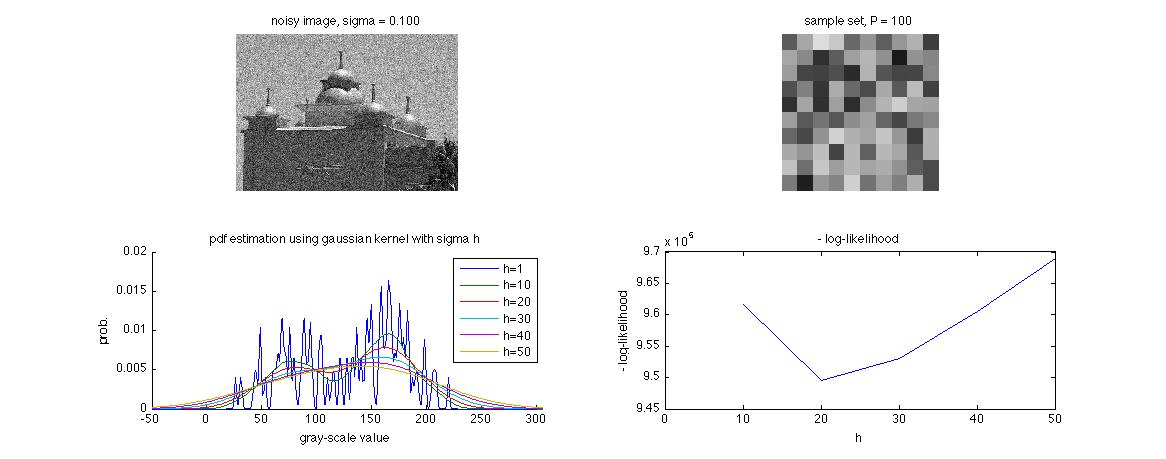
\includegraphics[width=0.8\textwidth]{plot100_01.jpg}
	\caption{caption}
	\label{sg:fig:plot100_01}
\end{figure}

\begin{figure}[h]
	\centering
		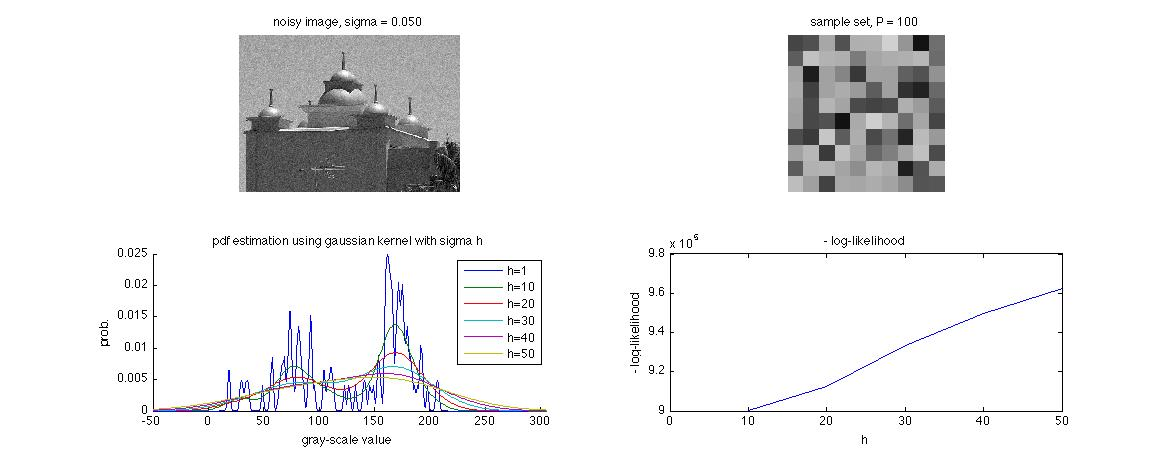
\includegraphics[width=0.8\textwidth]{plot100_005.jpg}
	\caption{caption}
	\label{sg:fig:plot100_005}
\end{figure}

\begin{figure}[h]
	\centering
		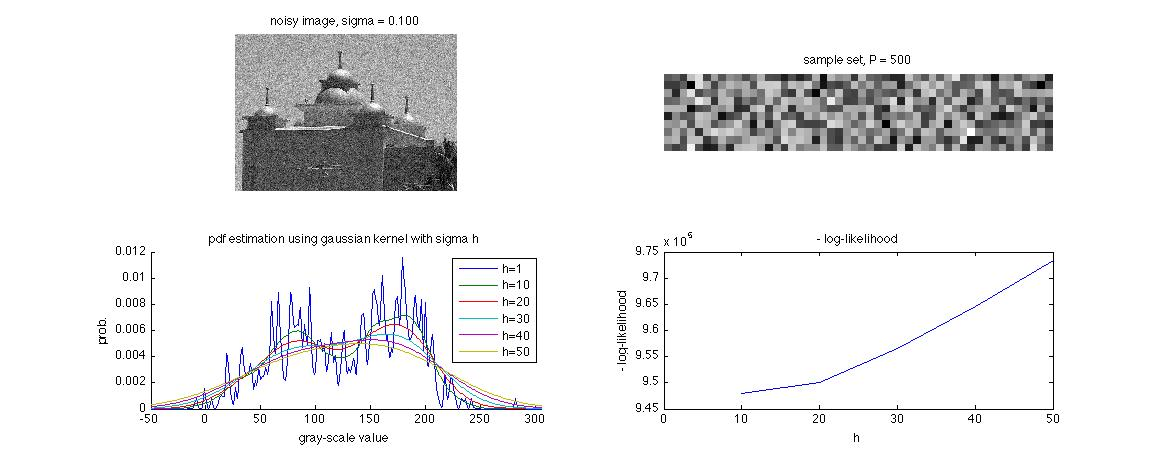
\includegraphics[width=0.8\textwidth]{plot500_01.jpg}
	\caption{caption}
	\label{sg:fig:plot500_01}
\end{figure}

\begin{figure}[h]
	\centering
		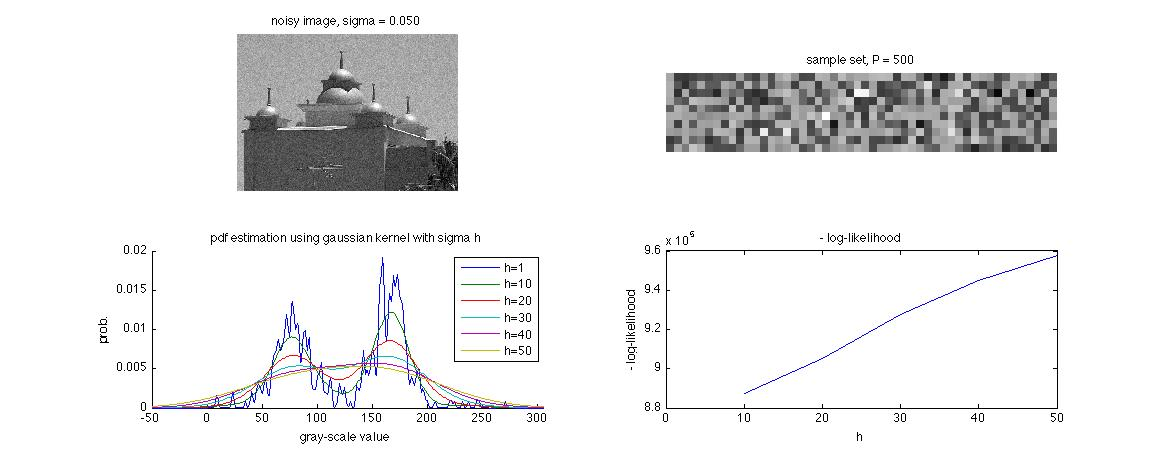
\includegraphics[width=0.8\textwidth]{plot500_005.jpg}
	\caption{caption}
	\label{sg:fig:plot500_005}
\end{figure}

\begin{figure}[h]
	\centering
		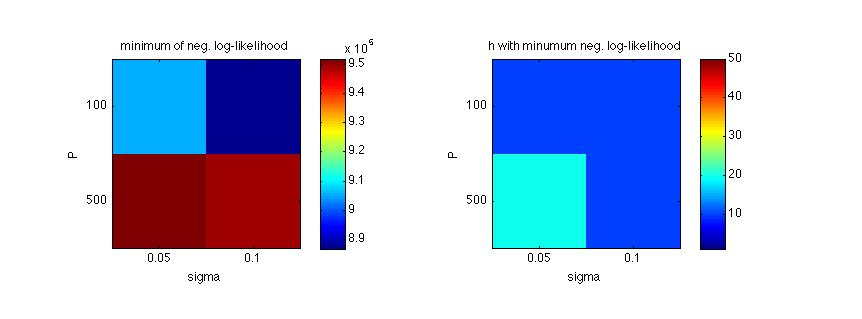
\includegraphics[width=0.8\textwidth]{best_log.jpg}
	\caption{caption}
	\label{sg:fig:best_log}
\end{figure}


\end{document}
